\chapter{Frames}\label{ch:frames}
A coordinate system is a reference framework that defines the position in either two- or three-dimensional space. In this chapter, the relationship between the coordinate system for the world and for the Cobra will be taken into account. A relationship between the robot and the world coordinates allows to go from the world coordinate to the robot. In figure \ref{fig:check_coordrobottoworld}, it is shown that the world coordinate is rotated and translated relative to the robot frame. 
\begin{figure}[hb]
  \centering
  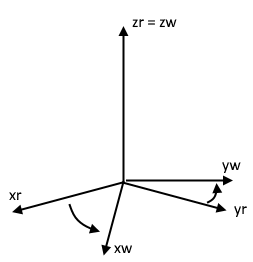
\includegraphics[width=3in]{figures/coordrobottoworld.png}
  \caption[Checkerboard and coordinate with robot to world] {Checkboard and coordinate with robot to world}
  \label{fig:check_coordrobottoworld}
\end{figure}

To transform the coordinate system from Robot to the World coordinates some calculations are needed. The following equation shows the relationship between the robot frame and the world frame.
\begin{align*}
\begin{bmatrix}
x_r \\
y_r \\
z_r \\
1 
\end{bmatrix}
= \underbrace{\begin{bmatrix}
a & b & x & c \\
d & e & x & f \\
g & h & x & i 
\end{bmatrix}}_{\text{R | T}}
\begin{bmatrix}
x_w \\
y_w \\
z_w\\
1 
\end{bmatrix}
\end{align*}
We assume that the z axis is on the same axis in both robot and world coordinate. The reason for this are that everything is measured in the XY plane. Therefore the above equation can we written as: 
\begin{align}
\begin{bmatrix}
x_r \\
y_r \\
1 
\end{bmatrix}
= \underbrace{\begin{bmatrix}
a & b & c \\
d & e & f \\
g & h & i 
\end{bmatrix}}_{\text{    R   | T}}
\begin{bmatrix}
x_w \\
y_w \\
1 
\end{bmatrix}
\label{eq:world_to_robot}
\end{align}

In order to find the coordinates $(x_r,y_r,z_r)$ in the robot frame, the matrix [R | T] and the coordinates in the world frame $(x_w,y_w,z_w)$ must be known. However, in this situation, only  the coordinates in the world frame were known. So, in order to find the robot coordinates in equation \ref{eq:world_to_robot}, the matrix [R | T] needs to be calculated. An easy way to find the solution of this issue would be to solve the [R | T] matrix as a system of equations. So that, if one point is known in the robot frame and in the world one, we will have three equations with nine unknowns. It is possible to observe these three equations with nine unknown between \ref{eq:system_of_equations1} and \ref{eq:system_of_equations2}.
 
\begin{align}
\label{eq:system_of_equations1}
x_r &= a\cdot x_w + b\cdot y_w + c \\
y_r &= d\cdot x_w + e\cdot y_w + f \\
1 &= g\cdot x_w + h\cdot y_w + i
\label{eq:system_of_equations2}
\end{align}
In order to solve this system, six more equations would be necessary to get the values of the [R | T] matrix. As a consequence, two more points would be essential to find nine different equations with nine unknown. 

The coordinates in the robot and world frames are measured by putting the robot manually at three different positions. To find the values of these points in the robot frame, a checkerboard is used as shown in figure \ref{fig:checkerboard}. 

\begin{figure}[h]
  \centering
  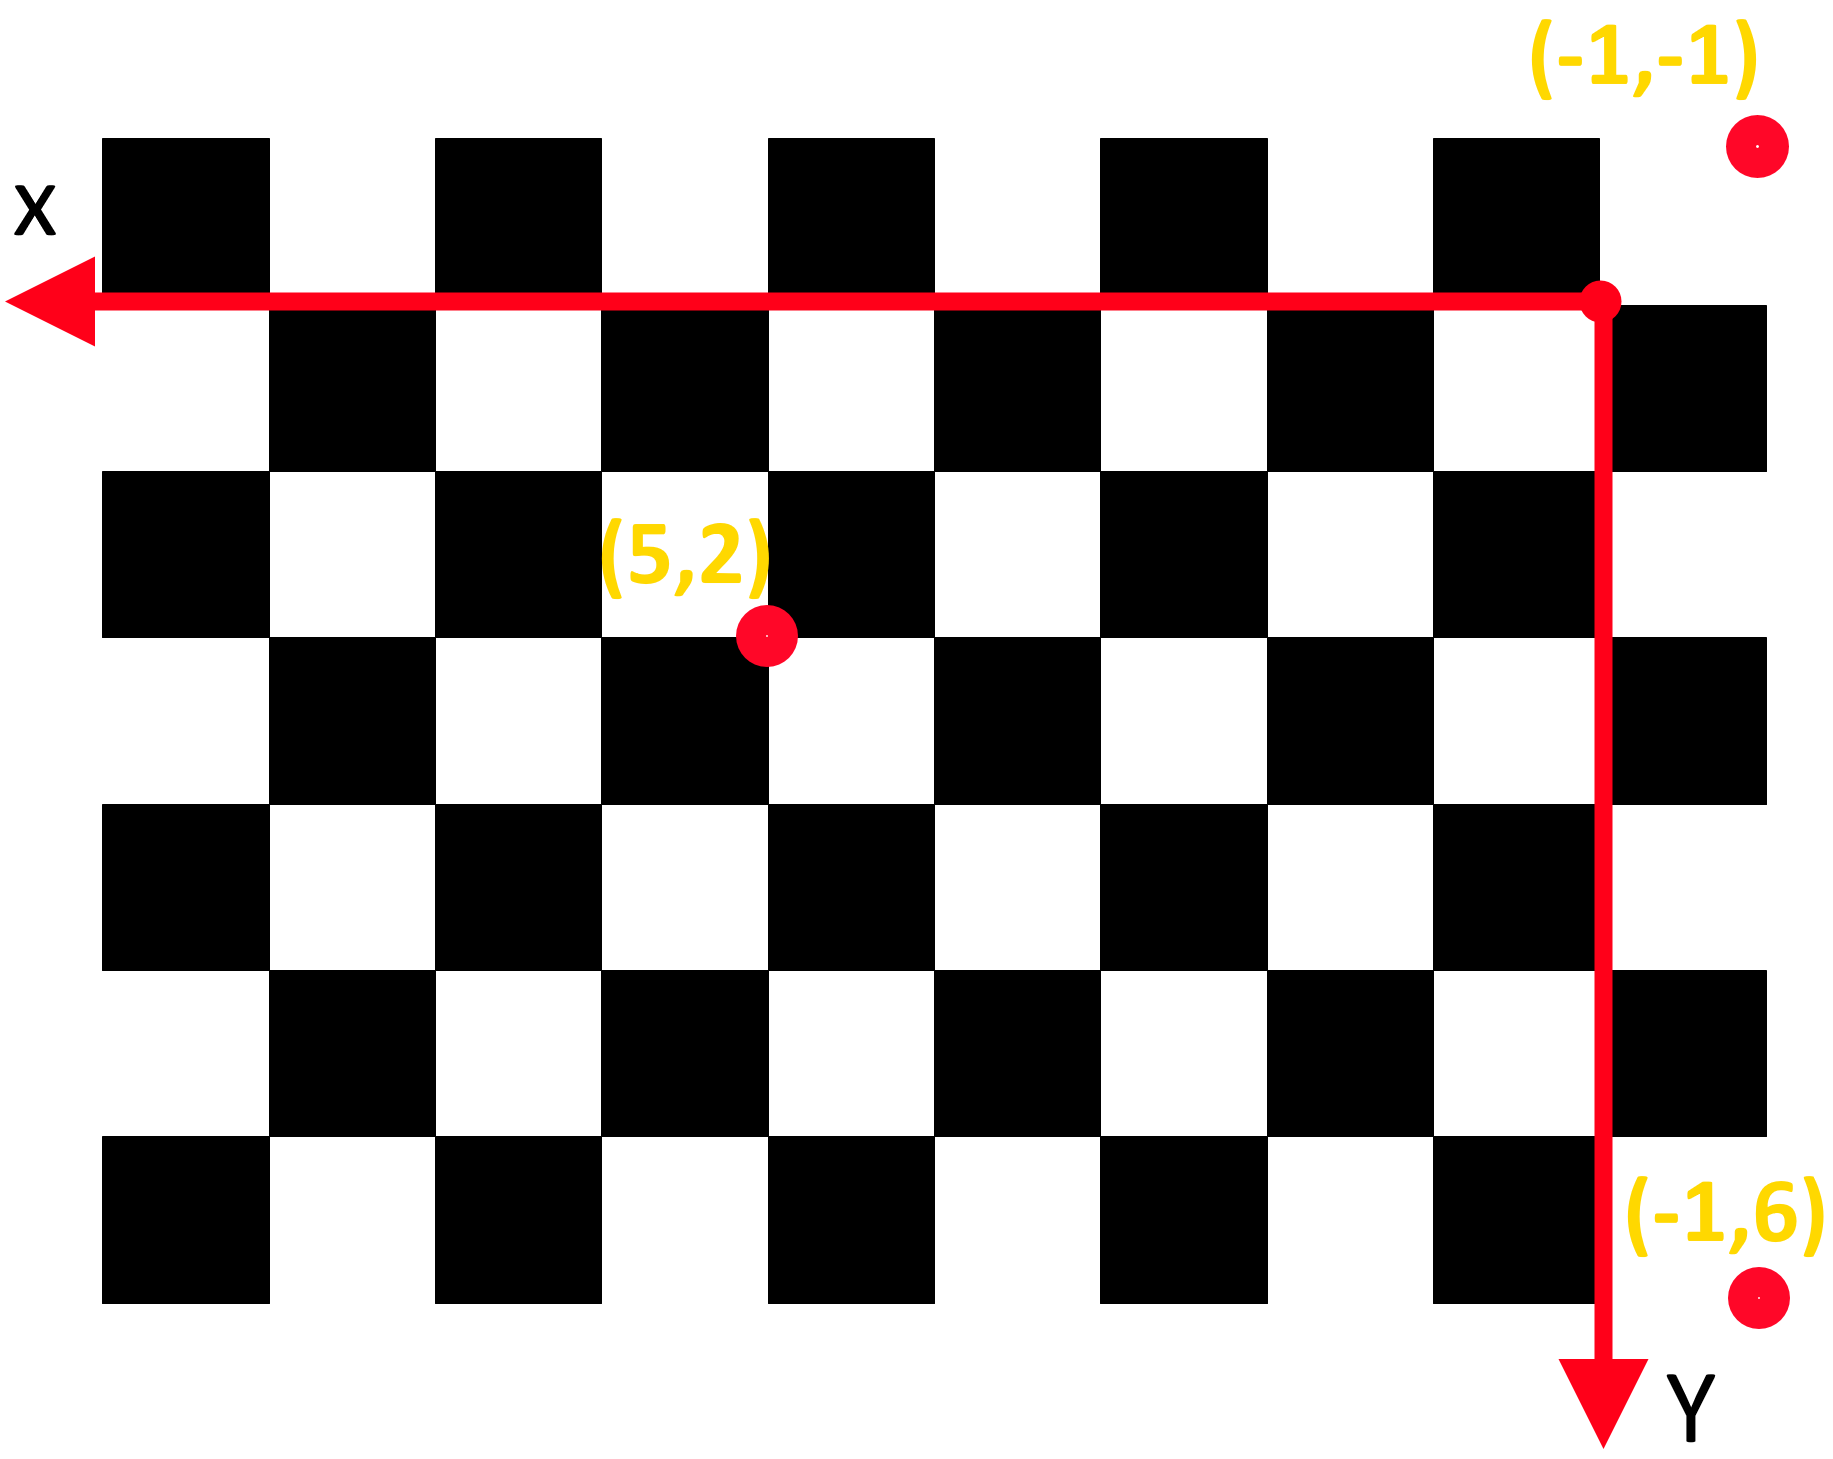
\includegraphics[width=2in]{figures/pattern.png}
  \caption[Checkerboard pattern] {Checkerboard pattern}
  \label{fig:checkerboard}
\end{figure}

The origin (0,0) is already known and from that it is possible to choose other two different positions. When these points are found, the nine different equations can be solved. The values of these three points are:

\begin{table}[h]
\begin{tabular}{| c | c | c | c |}
\hline
   & Point 1 & Point 2 & Point 3 \\
   \hline
  World & 28*[-1\quad -1] & 28*[-1\quad 6] & 28*[5\quad 2] \\
  Robot & [239.484\quad 198.714] & [233.953\quad 398.995]   & [408.578\quad 287.651] \\
  \hline
\end{tabular}
\end{table}

The 9 different equations will then be:
\begin{align*} 
p_1(x_r) &= a\cdot p_1(x_w) + b\cdot p_1(y_w) + c \\
p_1(y_r) &= d\cdot p_1(x_w) + e\cdot p_1(y_w) + f \\
1 &= g\cdot p_1(x_w) + h\cdot p_1(y_w) + k \\
p_2(x_r) &= a\cdot p_2(x_w) + b\cdot p_2(y_w) + c\\
p_2(y_r) &= d\cdot p_2(x_w) + e\cdot p_2(y_w) + f \\
1 &= g\cdot p_2(x_w) + h\cdot p_2(y_w) + k \\
p_3(x_r) &= a\cdot p_3(x_w) + b\cdot p_3(y_w) + c \\
p_3(y_r) &= d\cdot p_3(x_w) + e\cdot p_3(y_w) + f \\
1 &= g\cdot p_3(x_w) + h\cdot p_3(y_w) + k
\end{align*}
By solving these equations the [R | T] matrix is:
\begin{align*}
\text{(R|T)} = 
\begin{bmatrix}
1.0206 & -0.0282 & 267.2713 \\
0.0185 & 1.0218 & 227.8426 \\
0 & 0 & 1.0000 
\end{bmatrix}
\end{align*}

